`\chapter{Mechanics Investigated} \label{chap:mechanics}
	A brief summary of the mechanical principles used in analyzing the results of the data gathered during experimentation is contained in this chapter. Figure \ref{fig:3_Point_Bend} illustrates a standard 3-Point bend fixture setup and figures \ref{fig:fixture_unloaded} and \ref{fig:fixture_loaded} show the actual 3-point bend fixture when loaded and unloaded.
	
\begin{figure} [H]
\centering
	\caption{3-Point Bend}
	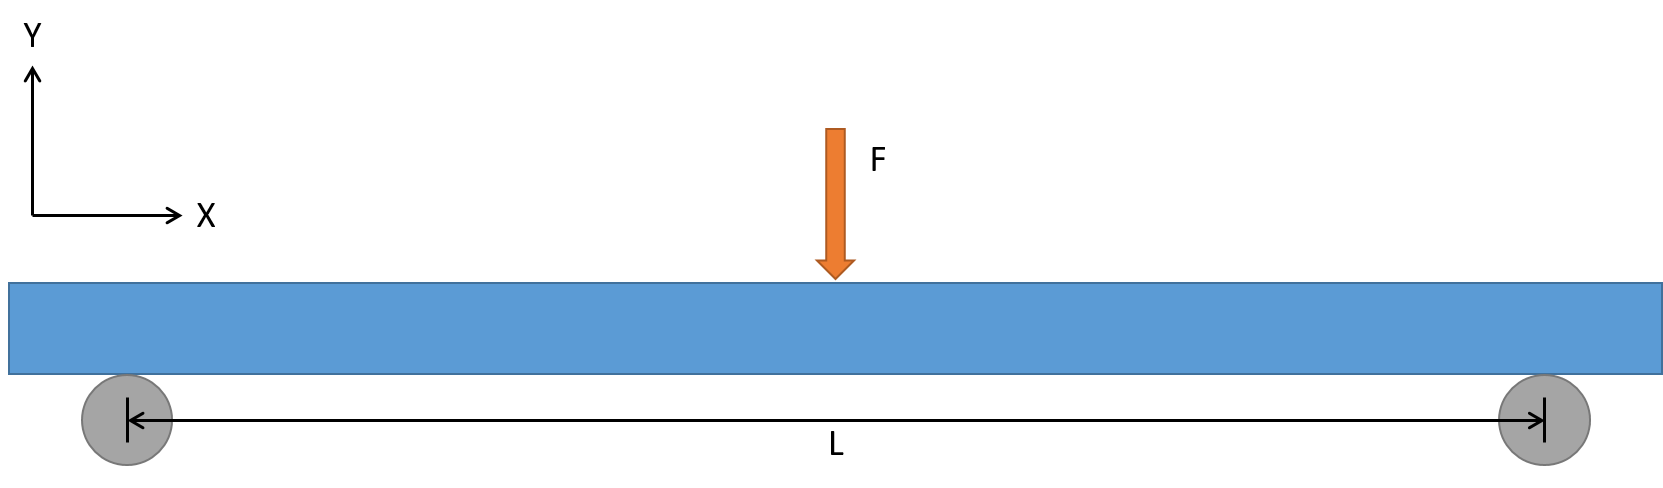
\includegraphics[width=\textwidth]{3_Point_Bend}
	\label{fig:3_Point_Bend}
\end{figure}



\begin{figure} [H]
\centering
	\caption{\label{ref_label_overall}3-Point Bend Fixture}
	\subfloat[Clamp without Bolts]{\label{fig:fixture_unloaded}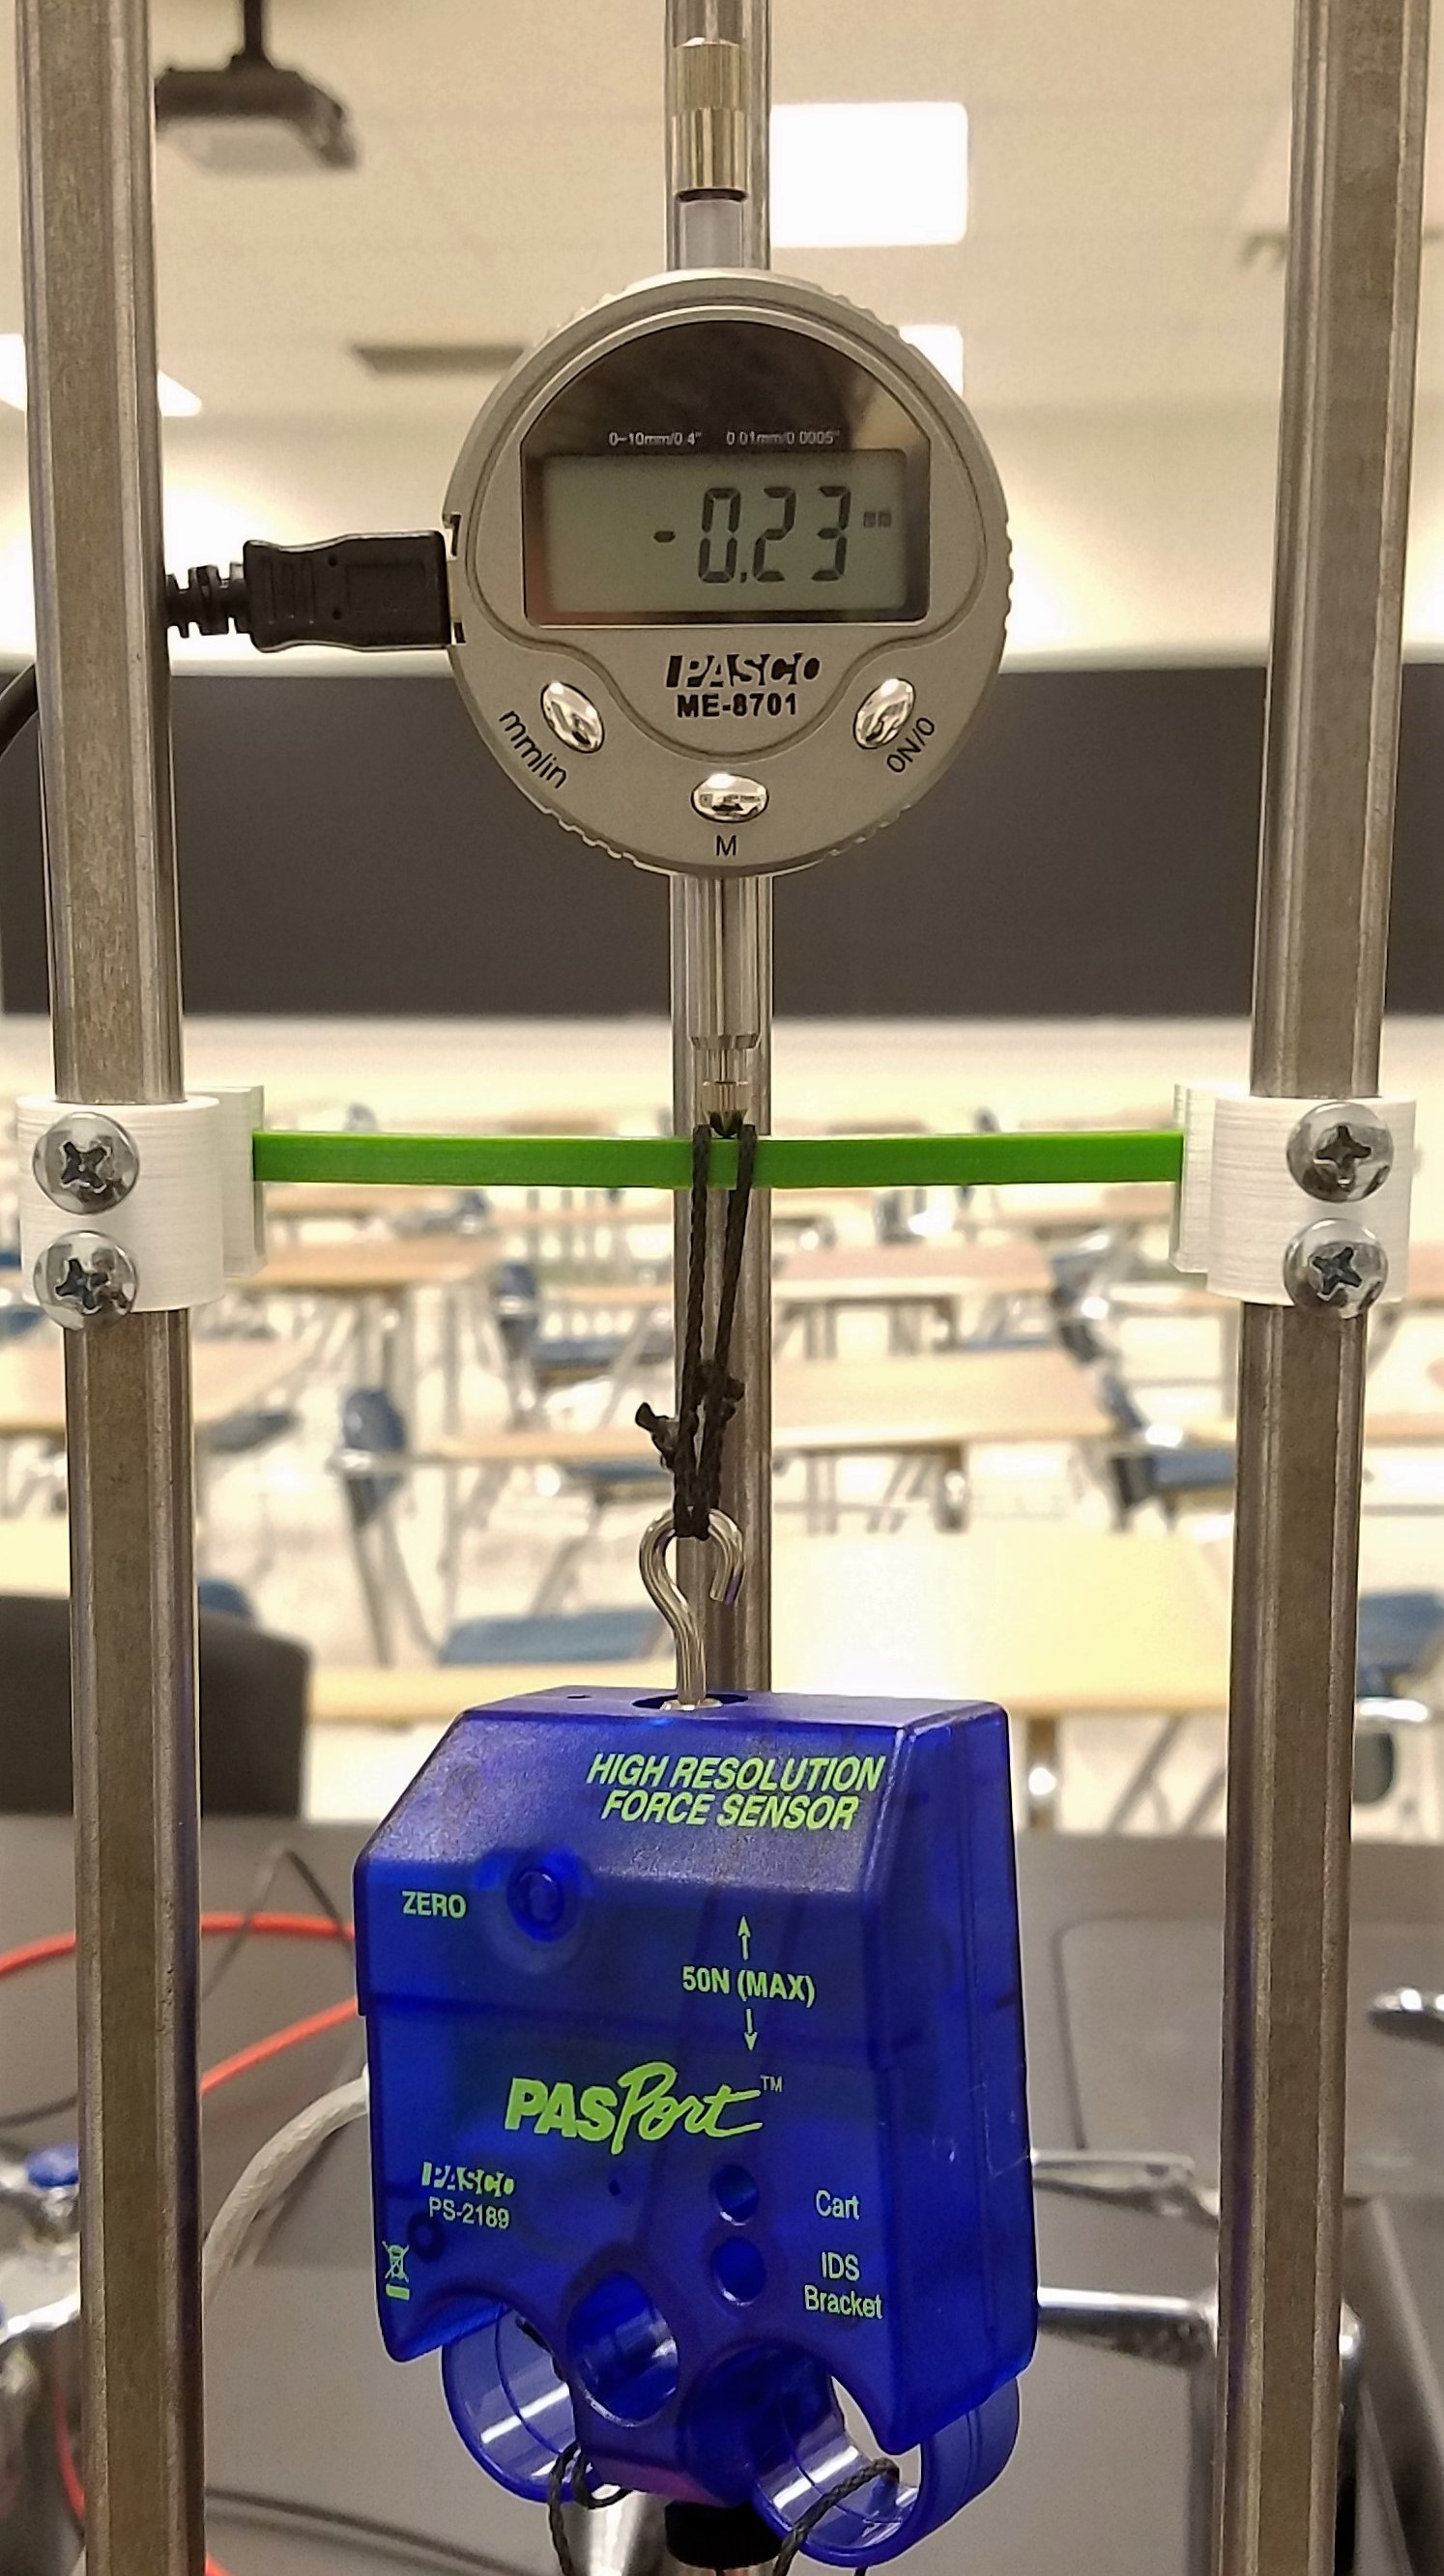
\includegraphics[height=12cm]{FIXTURE_RUNNING_UNLOADED}}\	
	\subfloat[Clamp without Bolts]{\label{fig:fixture_loaded}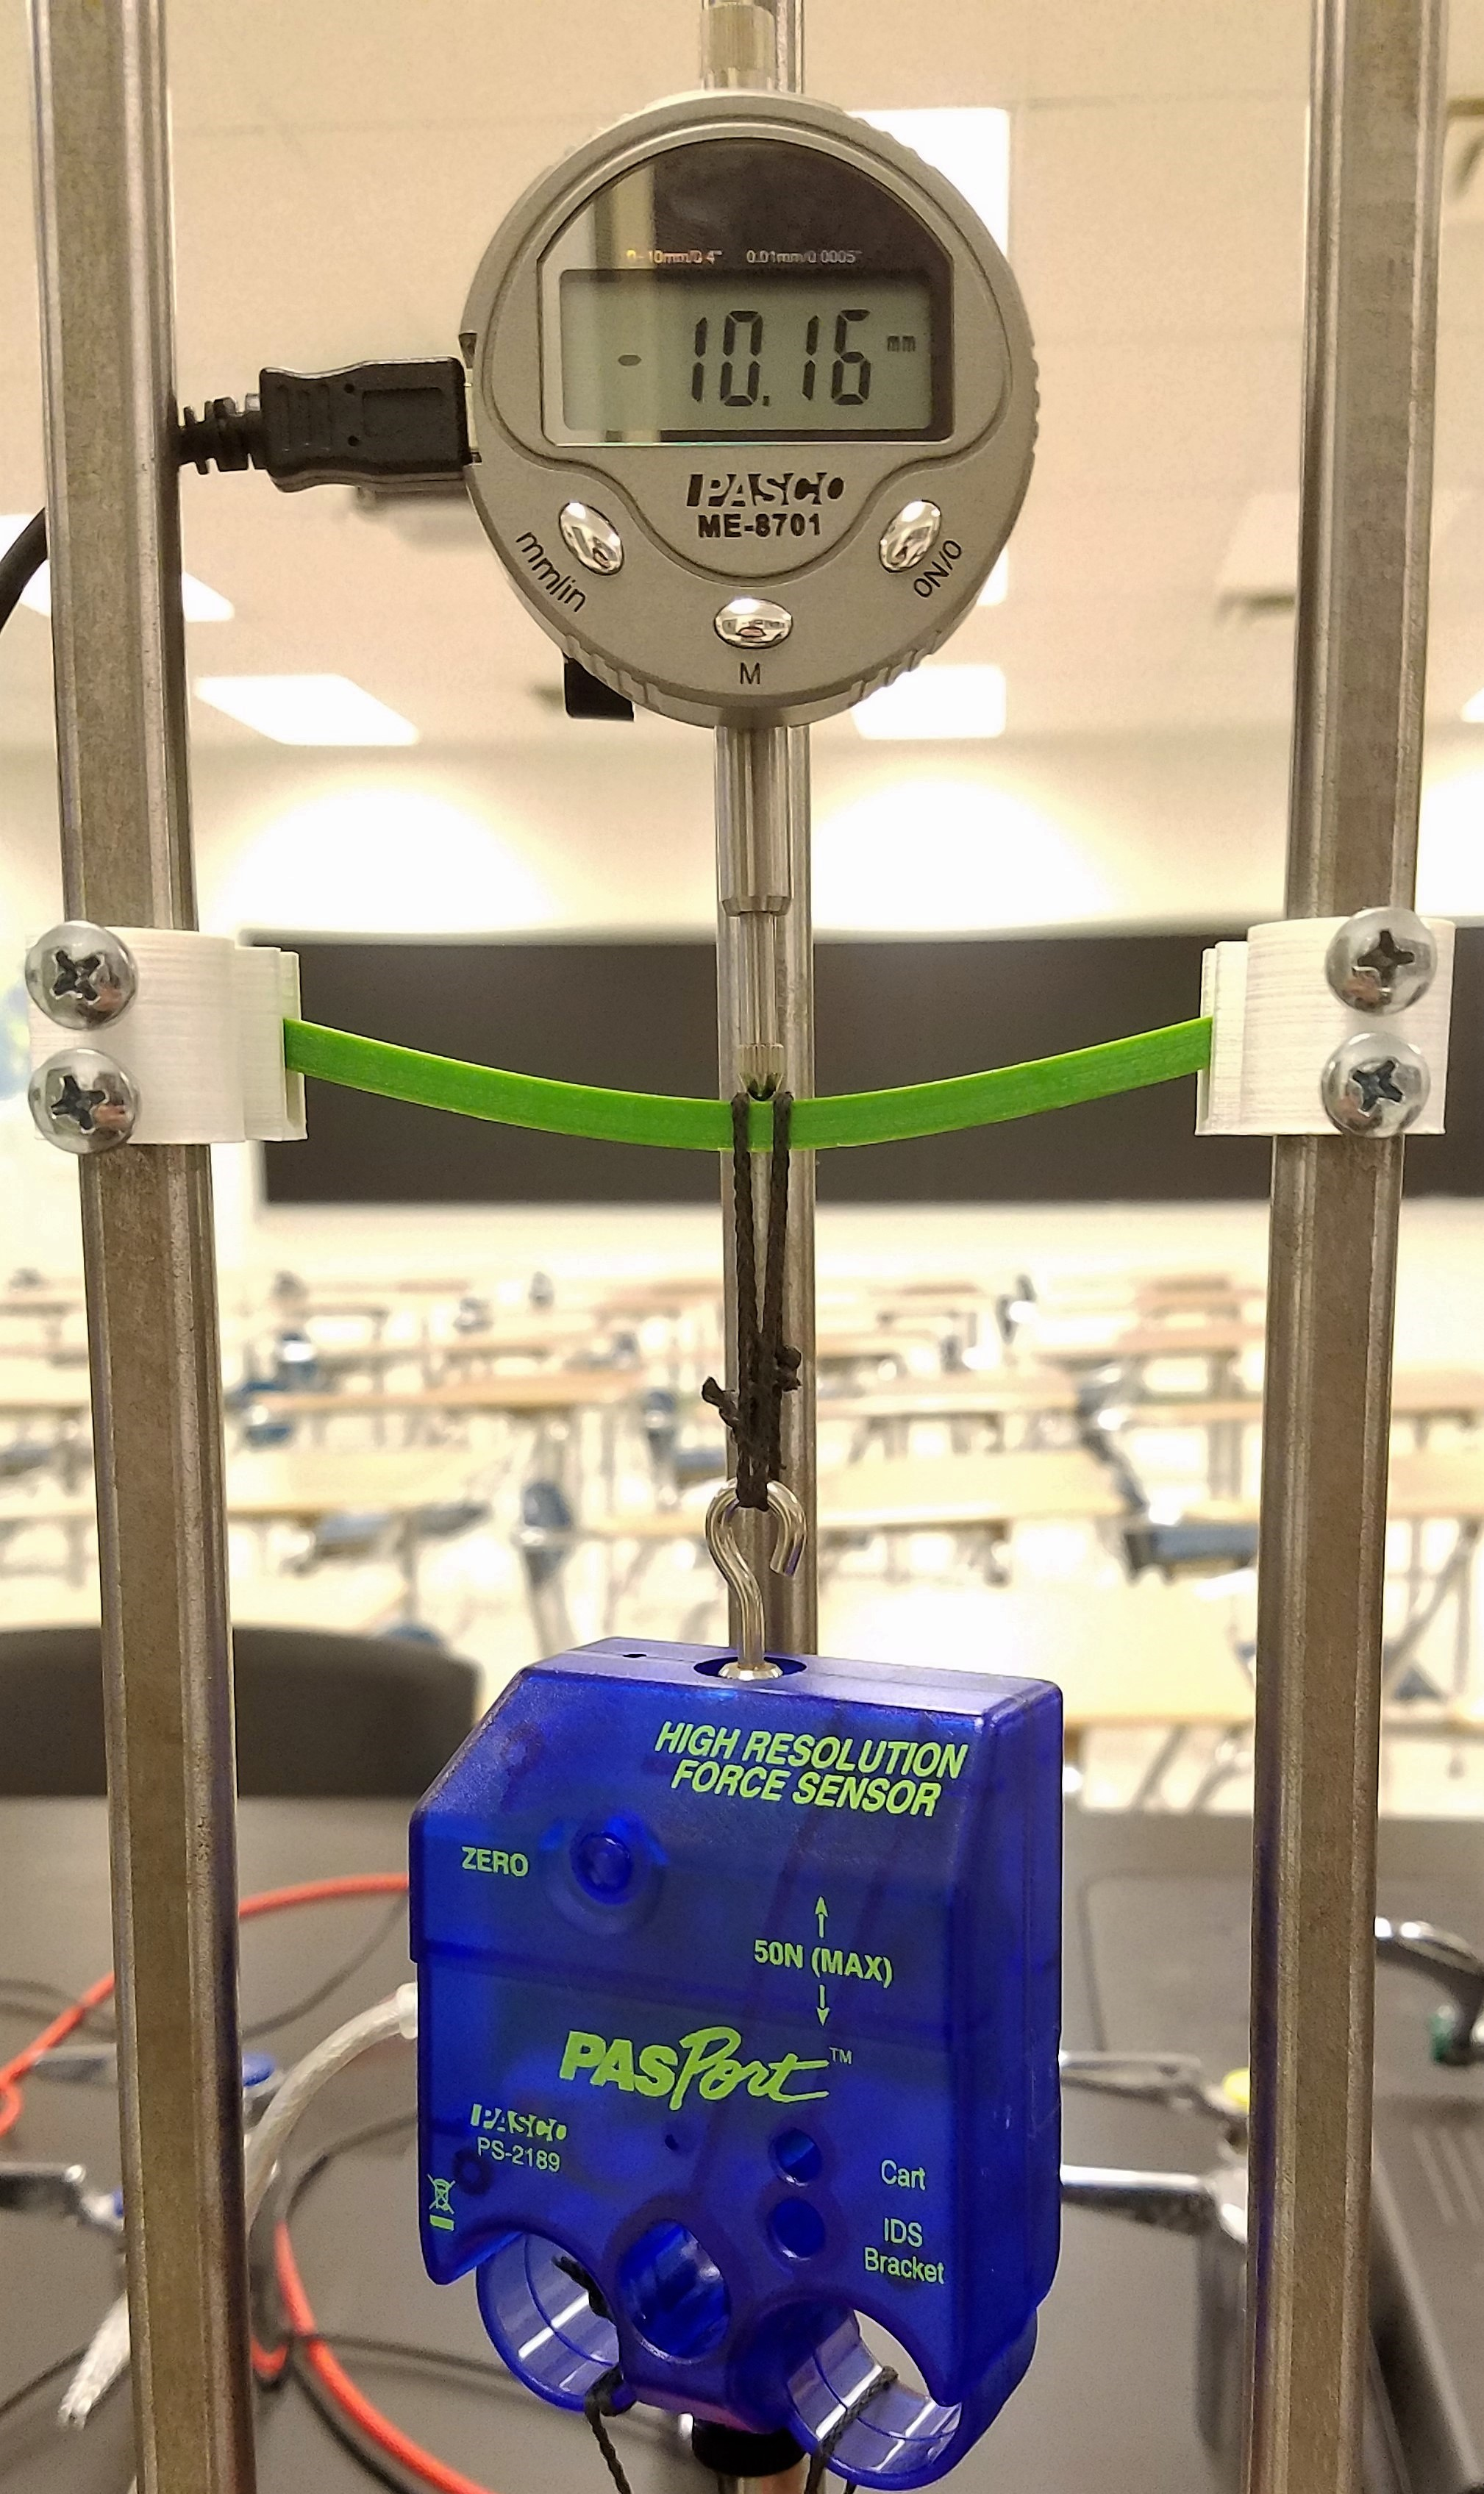
\includegraphics[height=12cm]{FIXTURE_RUNNING_LOADED}}\
\end{figure}

\section{Flexural Modulus of a Beam} \label{sec:modulus}
	With the test fixture being used we assume a beam supported by rollers on each side for our bending stress calculations. The equation below, taken from R.C. Hibbeler's book Statics and Mechanics of Materials, specifies the generalized equation for bending. The bending stress is characterized by the distance between supports, $d$, the height $h$, and width $w$ for the square and rectangular beams.

\begin{equation} \label{eq:1}
IE\frac{d^2v}{dx^2} = M(x)\quad \text{\citep{Hibbeler2010}}
\end{equation}

Assuming a beam supported by two rollers -- thus capable of lateral movement -- with a point force focused on the center of the beam, where $L$ is the distance between the two supports and $F$ is the force applied, the behavior of the beam can be described with the following equations.

\begin{equation} \label{eq:2}
IE\frac{d^2v_1}{dx^2} = Fx, \; 0 \leq x \leq \frac{L}{2}
\end{equation}
\begin{equation} \label{eq:3}
IE\frac{d^2v_2}{dx^2} = Fx, \; \frac{L}{2} \leq x \leq L
\end{equation}

Equations \ref{eq:2} \& \ref{eq:3} can then be integrated to obtain the following array of equations.

\begin{table} [h]
	\centering
	\begin{tabularx}{\textwidth}{| X X |}
	\multicolumn{2}{c}{\textbf{Bending Equations}} \\ \hline
	\vbox{\begin{equation} \label{eq:4} IE\frac{d^2v_1}{dx^2} = Fx \end{equation}} & \vbox{\begin{equation} \label{eq:7} IE\frac{d^2v_2}{dx^2} = Fx \end{equation}} \\
	\vbox{\begin{equation} \label{eq:5} IE\frac{dv_1}{dx} = \frac{1}{2}Fx^2 + C_1 \end{equation}} & \vbox{\begin{equation} \label{eq:8} IE\frac{dv_2}{dx} = \frac{1}{2}Fx^2 + C_3 \end{equation}}\\ 
	\vbox{\begin{equation} \label{eq:6} IEv_1 = \frac{1}{6}Fx^3 + C_1x + C_2  \end{equation}} & \vbox{\begin{equation} \label{eq:9} IEv_2 = \frac{1}{6}Fx^3 + C_3x + C_4 \end{equation}}\\ \hline
	\end{tabularx}
	\captionsetup{textformat=empty,labelformat=blank}
	\caption{Table of Bending Equations}
	\label{tab:bending}
\end{table}
\par

The following boundary conditions are assumed based on the behavior of the beam being supported on rollers at either end and having a point force applied in the center of the beam. Conditions \ref{bc:1} and \ref{bc:2} are assumed because the end points are constricted from vertical movement in the negative Y direction due to the rollers. shown by figure \ref{fig:3_Point_Bend}. The conditions \ref{bc:3} and \ref{bc:4} at $\frac{L}{2}$ are assumed because the deflection and rate of deflection are being measured at the same point from both ends.

\begin{table} [h]
	\centering
	\begin{tabularx}{\textwidth}{ | X  X | }
	\multicolumn{2}{c}{\textbf{Boundary Conditions}} \\ \hline
	\vbox{\begin{equation} \label{bc:1} v_1(0) = 0 \end{equation}} & \vbox{\begin{equation} \label{bc:2} v_2(L) = 0 \end{equation}} \\
	\vbox{\begin{equation} \label{bc:3} v_1\left(\frac{L}{2}\right) = v_1\left(\frac{L}{2}\right) \end{equation}} & \vbox{\begin{equation} \label{bc:4} \frac{dv_1}{dx}\vert_{\frac{L}{2}} = \frac{dv_1}{dx}\vert_{\frac{L}{2}} \end{equation}} \\ \hline
	\end{tabularx}
	\captionsetup{textformat=empty,labelformat=blank}
	\caption{Table of Boundary Conditions}
	\label{tab:bounds}
\end{table}
\par


While the boundary conditions can be applied to the equations in any order, for simplicity one start by applying boundary condition \eqref{bc:1} to \eqref{eq:6} to solve for $C_2$ and find that $C_2 = 0$. \eqref{eq:5} and \eqref{eq:8} can then be evaluated using boundary condition \eqref{bc:4} to determine $C_1 = C_3$ as shown below.

\begin{align*}
v_1(0) = 0; & \quad \frac{1}{6}F\cdot0 + C_1\cdot0 + C_2 = 0 \; \implies \; C_2 = 0 \\
\frac{dv_1}{dx}\vert_{\frac{L}{2}} = \frac{dv_1}{dx}\vert_{\frac{L}{2}}; & \quad \frac{F}{2}\left(\frac{L}{2}\right)^2 + C_1 = \frac{F}{2}\left(\frac{L}{2}\right)^2 + C_3 \; \implies \; C_1 = C_3 \\
\end{align*}

Following this, evaluating \eqref{eq:6} and \eqref{eq:9} with the boundary condition \eqref{bc:3} further simplifies the set of equations by showing that $C_4 = 0$.

\begin{align*}
v_1\left(\frac{L}{2}\right) = v_1\left(\frac{L}{2}\right); & \quad  \frac{F}{6}\left(\frac{L}{2}\right)^3 + \frac{C_1L}{2} = \frac{F}{6}\left(\frac{L}{2}\right)^3 + \frac{C_1L}{2} + C_4 \; \implies \; C_4 = 0
\end{align*}

Finally, one can apply the boundary condition \eqref{bc:2} to \eqref{eq:9}.

\begin{align*}
v_2 = 0; & \quad \frac{FL^3}{6} + C_1L = 0 \; \implies \; C_1 = -\frac{FL^2}{6}
\end{align*}

By applying these solutions, equations \eqref{eq:6} and \eqref{eq:9} become the following:

\begin{align*}
v_1(x) = \frac{F}{6IE}(x^3 - L^2x) = v_2
\end{align*}

Now, one can conclude that $v_1 = v_2$ and simply use the following equation to determine the displacement of a beam in a 3-point bend fixture.

\begin{equation} \label{eq:10}
v(x) = \frac{F}{6IE}(x^3 - L^2x)
\end{equation}

Because a symmetrical bending experiment is being performed with a point load centered directly at $\frac{L}{2}$, this equation can be evaluated at the midpoint to come up with a solution for a three point bend test consisting of a beam on two rollers and a force applied at the center.

\begin{align}
v\left(\frac{L}{2}\right) = \frac{F}{6IE}\left[\left(\frac{L}{2}\right)^3 - \frac{L^3}{2}\right] \nonumber \\
v\left(\frac{L}{2}\right) = \frac{F}{6IE}\left[\frac{L^3}{8} - \frac{L^3}{2}\right] \nonumber \\
\label{eq:v} v\left(\frac{L}{2}\right) = \frac{FL^3}{48IE}
\end{align}

Knowing this, and substituting in $I = \frac{1}{12}bh^3$ we can rearrange our formula for finding the modulus of elasticity as long as our bend point stays centered.

\begin{equation}\label{eq:modulus}
E(F,L,b,h,v) = \frac{FL^3}{4vbh^3}
\end{equation}
Equation \eqref{eq:modulus} will be used in calculations for determining the modulus of elasticity of PLA and ABS square and rectangular beams using experimental data collected. The method of data collection and test setup will be explained in chapter 4. The table below outlines each of the variables significance and how they will be measured.

\begin{table} [h]
	\centering
	\begin{tabularx}{\textwidth}{ l | l | X}
		\multicolumn{3}{c}{\textbf{\eqref{eq:modulus}Variable Descriptions}} \\ \hline
		E & Modulus of Elasticity & Calculated using \eqref{eq:modulus}\\
		L & Distance between beam supports & Measured using calipers.\\
		b & Base of beam cross section & Measured using calipers. \\
		h & Height of beam cross section & Measured using calipers.\\
		F & Force applied & Measured using PASCO force sensor. \\
		v & Displacement & Measured using PASCO displacement gauge. \\
	\end{tabularx}
	\label{tab:variables}
	\captionsetup{textformat=empty,labelformat=blank}
	\caption{Table of Variables for \eqref{eq:modulus}}
\end{table}
\par
The length of the beams will remain constant based on the test fixture. The width and height of the beams were measured at both end points and midpoint and then averaged to obtain the figures that were used in calculations of the elastic modulus. The beam measurements are included in Appendices \ref{app:square} and \ref{app:rectangle}.

\section{Square and Rectangular Beam Uncertainty}
The uncertainty of estimating the behavior of a beam was calculated according to equation \ref{eq:sq_rect_uncertainty}. The uncertainty in predicting the behavior of the Square and Rectangular beams is important to observe and record as it provides insight as to how one would design a structure and the variance in strength that would be expected. $F_{Predicted}$ is defined as the force calculated to bend the beam to a randomly chosen deflection within the linear elastic region. $F_{Actual}$ is the actual force that applied to bend the beam to that deflection amount during experimentation.

\begin{equation}\label{eq:sq_rect_uncertainty}
U = 100*\frac{F_{Predicted}-F_{Actual}}{F_{Actual}}
\end{equation}

\section{I-Beam Predictions}
Based on the results for the Modulus of Elasticity of both ABS and PLA specimens, an Excel spreadsheet was used to determine the moment of inertia and potential strength of a 100\% fill I-beam when given dimensions of the top, web and bottom of the beam. Appendix \ref{app:ibeams}\par
	The beams' predicted deformation is calculated by first finding the moment of inertia of the cross-sectional area of the beam and then inserting it into the following equation from \ref{sec:modulus}. 

\begin{equation}
v = \frac{FL^3}{48IE}
\end{equation}

\section{PLA I-Beam Uncertainty}
The uncertainty of estimating the behavior of the I-beams was calculated according to equation \ref{eq:ib_uncertainty}. $v_{Predicted}$ is the amount of deflection that one would expect to see when applying a 40N load to the midpoint of the beam and $v_{Actual}$ is the observed deflection when 40N is applied.

\begin{equation}\label{eq:ib_uncertainty}
U = 100*\frac{v_{Predicted}-v_{Actual}}{v_{Actual}}
\end{equation}